\subsection{Thời gian: Nguyên thủy thời gian – Tức thời}
CareCruiser [163] là một hệ thống trực quan hỗ trợ việc xác định sơ bộ ảnh hưởng của các hoạt động lâm sàng đối với tình trạng của bệnh nhân. Để đạt được mục tiêu này, CareCruiser trực quan hóa các chi tiết trong pháp đồ điều trị kết hợp với các thông số của bệnh nhân, đặc biệt là thông số liên quan đến các quá trình diễn tiến thay đổi theo thời gian. Nó hỗ trợ khai phá thông tin thông qua việc căn chỉnh, đánh dấu màu, lọc và cung cấp thông tin về bối cảnh chung cũng như thông tin chi tiết cần tập trung. Sắp xếp các kế hoạch điều trị lâm sàng theo chiều dọc sẽ giúp đơn giản hóa việc so sánh hiệu quả của các phương pháp điều trị khác nhau hoặc so sánh hiệu quả khác nhau của cùng một phương pháp điều trị nhưng trên nhiều đối tượng bệnh nhân khác nhau. Bên cạnh đó, việc theo dõi hiệu quả của một hoạt động lâm sàng trong tất cả các lần thực hiện (ví dụ: sử dụng lặp lại một loại thuốc nhất định) sẽ giúp tạo điều kiện thuận lợi cho việc so sánh hiệu quả của hoạt động lâm sàng này đối với tình trạng của bệnh nhân. Ba cách phối màu khác nhau được sử dụng để làm nổi bật các phần thú vị trong quá trình phát triển một tham số: việc làm nổi bật (tô đậm) khoảng cách giữa các giá trị thực tế với giá trị dự kiến giúp xác định các giá trị quan trọng; việc làm nổi bật (tô đậm) tiến trình của các giá trị thực tế so với các giá trị ban đầu cho thấy kế hoạch điều trị được áp dụng có tác dụng như đạt mức độ nào so với mong đợi; và việc làm nổi bật độ dốc (sự thay đổi đột ngột) của một giá trị sẽ giúp ta khám phá những tác động tức thời của các hoạt động lâm sàng được áp dụng. Một thanh trượt được cung cấp để lựa chọn màu sắc làm nổi bật cho các sự kiện được chọn (xem Hình (\ref{fig:f7.10}), phía trên cùng) và một cửa sổ cung cấp hình ảnh đã làm mờ thông tin màu bên ngoài đường viền được sử dụng để hỗ trợ quan sát tập trung vào một vùng cần quan tâm cụ thể (ví dụ: phần thời gian nhất định sau khi áp dụng một hành động lâm sàng). Các vùng ít được nhấn mạnh hơn một chút bên ngoài cửa sổ đã nêu trên biểu thị đường cong các giá trị liên tiếp của hoạt động, từ đó cung cấp một số thông tin ngữ cảnh xung quanh cho các giá trị nổi bật mà chúng ta đang quan tâm phân tích. 
\begin{figure}[H] % places figure environment here   
    \centering % Centers Graphic
    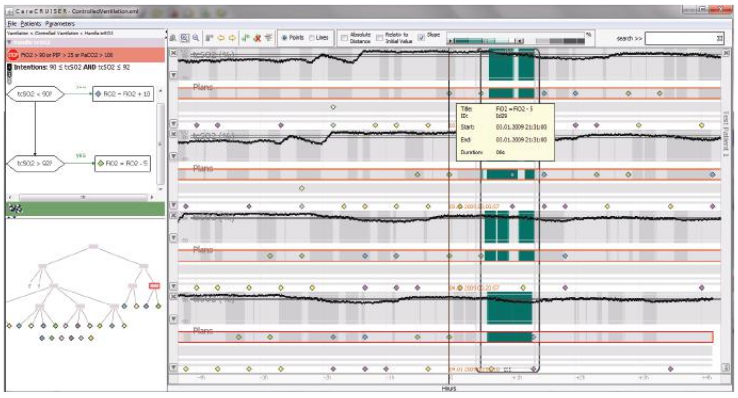
\includegraphics[width=0.8\textwidth]{assets/fig_7_10.png} 
    \caption{CareCruiser [163]. Chế độ xem theo thời gian (ở phía bên phải) sắp xếp các thông số của bệnh nhân cùng với các hoạt động lâm sàng đã được thực hiện (các chấm nhỏ bên dưới biểu đồ đường) dọc theo trục thời gian nằm ngang. Các chế độ xem theo trật tự móc nối logic và trật tự phân cấp ghi lại các kế hoạch điều trị được hiển thị ở phía bên trái. Khu vực đang được chọn ở cửa sổ bên phải thể hiện giá trị tcSO2 của bệnh nhân giảm chậm sau khi áp dụng một hoạt động lâm sàng cụ thể. (Nguồn: Thực hiện bằng phần mềm nguyên mẫu CareCruiser.)} % Creates caption underneath graph
    \label{fig:f7.10}
\end{figure}